% Options for packages loaded elsewhere
\PassOptionsToPackage{unicode}{hyperref}
\PassOptionsToPackage{hyphens}{url}
\PassOptionsToPackage{dvipsnames,svgnames,x11names}{xcolor}
\documentclass[
  american,
  11pt,
  letterpaper,
]{article}
\usepackage{xcolor}
\usepackage[margin=1in]{geometry}
\usepackage{amsmath,amssymb}
\setcounter{secnumdepth}{-\maxdimen} % remove section numbering
\usepackage{iftex}
\ifPDFTeX
  \usepackage[T1]{fontenc}
  \usepackage[utf8]{inputenc}
  \usepackage{textcomp} % provide euro and other symbols
\else % if luatex or xetex
  \usepackage{fontspec}
  \defaultfontfeatures{Scale=MatchLowercase}
  \defaultfontfeatures[\rmfamily]{Ligatures=TeX,Scale=1}
\fi
\usepackage{lmodern}
\ifPDFTeX\else
  % xetex/luatex font selection
  \setmainfont[]{Times New Roman}
\fi
% Use upquote if available, for straight quotes in verbatim environments
\IfFileExists{upquote.sty}{\usepackage{upquote}}{}
\IfFileExists{microtype.sty}{% use microtype if available
  \usepackage[]{microtype}
  \UseMicrotypeSet[protrusion]{basicmath} % disable protrusion for tt fonts
}{}
\makeatletter
\@ifundefined{KOMAClassName}{% if non-KOMA class
  \IfFileExists{parskip.sty}{%
    \usepackage{parskip}
  }{% else
    \setlength{\parindent}{0pt}
    \setlength{\parskip}{6pt plus 2pt minus 1pt}}
}{% if KOMA class
  \KOMAoptions{parskip=half}}
\makeatother
\usepackage{graphicx}
\makeatletter
\newsavebox\pandoc@box
\newcommand*\pandocbounded[1]{% scales image to fit in text height/width
  \sbox\pandoc@box{#1}%
  \Gscale@div\@tempa{\textheight}{\dimexpr\ht\pandoc@box+\dp\pandoc@box\relax}%
  \Gscale@div\@tempb{\linewidth}{\wd\pandoc@box}%
  \ifdim\@tempb\p@<\@tempa\p@\let\@tempa\@tempb\fi% select the smaller of both
  \ifdim\@tempa\p@<\p@\scalebox{\@tempa}{\usebox\pandoc@box}%
  \else\usebox{\pandoc@box}%
  \fi%
}
% Set default figure placement to htbp
\def\fps@figure{htbp}
\makeatother
\ifLuaTeX
\usepackage[bidi=basic,shorthands=off]{babel}
\else
\usepackage[bidi=default,shorthands=off]{babel}
\fi
\ifPDFTeX
\else
\babelfont{rm}[]{Times New Roman}
\fi
\ifLuaTeX
  \usepackage{selnolig} % disable illegal ligatures
\fi
\setlength{\emergencystretch}{3em} % prevent overfull lines
\providecommand{\tightlist}{%
  \setlength{\itemsep}{0pt}\setlength{\parskip}{0pt}}
\usepackage{fancyhdr}
\usepackage{enumitem}
\usepackage{caption}
\usepackage{bm}
\usepackage{float}
\usepackage{microtype}
\usepackage{xurl}
\usepackage{ragged2e}

\pagestyle{fancy}
\fancyhf{}
\fancyfoot[C]{\thepage}
\renewcommand{\headrulewidth}{0pt}

\setlength{\parindent}{0pt}
\setlength{\parskip}{6pt plus 2pt minus 1pt}
\setlist{nosep,leftmargin=*}
\captionsetup{font=small,labelfont=bf}
\setlength{\emergencystretch}{3em}
\sloppy
\hyphenation{im-ple-men-ta-tion op-er-a-tion-al-i-za-tion}


\usepackage{amsmath,amssymb,graphicx}
\renewcommand{\familydefault}{\rmdefault}
\setcounter{secnumdepth}{0}
\usepackage{etoolbox}
\AtBeginEnvironment{longtable}{\small}
\usepackage{bookmark}
\IfFileExists{xurl.sty}{\usepackage{xurl}}{} % add URL line breaks if available
\urlstyle{same}
\hypersetup{
  pdfauthor={Micah Blumberg},
  pdflang={en-US},
  colorlinks=true,
  linkcolor={blue},
  filecolor={Maroon},
  citecolor={Blue},
  urlcolor={blue},
  pdfcreator={LaTeX via pandoc}}

\author{}
\date{}

\begin{document}

\begin{center}
{\LARGE\bfseries Temporal Ensembles in Self-Aware Networks: Dendritic Recovery, Phase-Structured Recurrence, and the Hypothesis of Temporal Experience\par}
\vspace{0.6em}
Micah Blumberg\par
Self Aware Networks Research Institute\par
\url{https://doi.org/10.5281/zenodo.23509960}
\end{center}

20 October 2026. \textbf{Paper 113 - Public preprint v1.2 - Not peer reviewed.} Public v1.0 (23 September 2026) and v1.1 (18 October 2026) remain unchanged. Version 1.1 added the temporal-selection comparison and its conditional constraints. This focused update adds three verified 2022 historical sources and clarifies their relationship to the later experiment. Existing mathematics, applications, figures and prospective tests are retained; no new neural data or physiological fit is reported.

\subsection{Abstract}\label{abstract}

A neural rendering must connect events across time without erasing the order or ownership of their contents. I propose a Temporal Ensemble Hypothesis: receiving components whose recent activity changes their readiness can contribute in a coordinated sequence while the effects of earlier contributions remain available. A three-branch alternating image motivates the hypothesis but is not assumed to be a universal rule. I distinguish activation, recovery, retained content, coupling, downstream use, and the further claim of elementary cellular temporal experience. Under explicit hard-window assumptions, a regular schedule of \emph{n} branches with recovery interval \emph{R} can sustain an overlap of \emph{k} distinct contributions with trace lifetime \emph{M} only when \emph{n} is at least \emph{k} and \emph{nM} is at least \emph{(k−1)R}. An imposed-schedule model checks that boundary; a readiness-plus-competition toy produces a three-branch cycle under one parameter setting. A passive-I/O comparison shows that an alternating route and a one-unit ordered-history route agree on all 27 declared input sequences. A further matched-logical-intervention control agrees on all 216 input/mask cases. A fifth local-state construction has competitive activation, adaptation and decaying object-feature traces. It retains all 576 separated-event orders and all 720 supplied ownership assignments in its fixed noiseless grid. However, an ordinary nonoscillatory state bank gives the same downstream outputs: shared linear trace decay and normalized input allocation make the aggregate independent of alternation. These deliberately elementary constructions establish feasibility, actual content use in a program and identification limits, not biological oscillation, route necessity or consciousness. I propose independently localized cellular and network perturbations to test whether the candidate timing relation contributes beyond generic state dependence. Temporal computation, whole-network experience, and the proposed elementary experience of a cell remain separate conclusions. A new state-resolved perceptual comparison motivates separate tests of represented content, selective downstream use and retained continuity; it does not identify a universal oscillation or the proposed cellular mechanism.

\subsection{1. The temporal problem inside SAN}\label{the-temporal-problem-inside-san}

The self-world construction described by Self Aware Networks is not a sequence of isolated pictures. Sound, movement, bodily condition, remembered significance and possible action are jointly usable because current activity is affected by what preceded it. Yet merely pooling nearby activity would erase distinctions. The sequence A--B--C and its reversal contain the same elements but can demand different predictions or actions. Two objects can occupy the same short interval without sharing a color or a trajectory. A mechanism of continuity must therefore retain selected earlier relations while protecting their order and ownership.

My starting image was three dendritic branches taking turns. One was active while another was changed by its previous activation and a third was preparing to contribute. At a larger scale I pictured cell groups coordinating in a similarly staggered way. I also asked whether an individual neuron's simple changing state could constitute an elementary temporal experience, analogized to one changing pixel in a larger display. These ideas motivated this paper, but they are not one claim. Branches can have history-dependent responsiveness without forming a triplet; networks can process sequences without oscillating; neither operation alone establishes experience.

The bird-and-cage thaumatrope introduces the integration question: two sequential presentations can contribute to one perceived relation. It is not evidence that the percept depends on three dendritic branches. The companion question is when the brain should \emph{not} merge presentations. That paired demand---continuity with differentiation---defines the functional target here.

This question has a SAN history that I should not compress into a claim of sudden novelty. In a note internally dated 21 September 2011, I joined sensation, learned statistical memory/prediction, neural activity, action and returned sensation, then called the self ``a learning loop that learns itself'' {[}9{]}. That is an embodied recurrent-system claim, not the later three-branch mechanism or proof of cellular experience. The present archive copy also appends a January 2023 transformer-paper excerpt; I do not assign that later text to 2011. A separate cutlet note repeats and extends parts of the earlier dialogue {[}10{]}, but is a derivative witness rather than a second independent 2011 source.

In an April 2012 note, I described cells as both playing and listening to a continuing ``song'' of activity in a learning feedback loop {[}6{]}. A September 2012 note placed nested learning loops, expectation and a possible dissipative input--output--structure cycle in the same conceptual family {[}7{]}. An undated note, preserved in the source archive by 2022, contemplated sequences of oscillating arrays, phase coincidence, inhibition, alternating decoherence and a possible splay state {[}8{]}. That last note also contains speculative cross-domain analogies; I use this narrow passage to recover the \emph{author's prior question}, not as physiological evidence or as a physics premise. None of these passages proposes a universal three-branch firing rule, measures branch recovery or establishes cellular experience. The present 2026 image gives the older embodied and temporal themes a more specific, testable compartment-level conjecture. The \href{https://github.com/v5ma/v5ma.github.io/blob/f6d3867df89ae9dea32f763b1d55c84212c41cc6/papers/companions/five-papers-20260923/temporal/paper/SOURCE-AND-NONDUPLICATION.md}{source and date ledger} separates owner-stated dates, local hashes, later custody and the current hypothesis.

\subsubsection{1.1 The 2022 records of interleaving and selective access}\label{the-2022-records-of-interleaving-and-selective-access}

A transcript in the Git version dated 8 June 2022 makes the temporal proposal explicit: ``You could interlace them so that they don't appear at the same time'' {[}24{]}. Its surrounding argument concerns sound, visual representations and multiple scales of detail recurring quickly enough to appear overlaid rather than successive. The recording catalogue assigns the underlying talk to 17 September 2021; the exact wording checked here is the June 2022 transcript, not a newly auditioned 2021 recording.

Two records dated 28 November 2022 join this interleaving idea to recurrence and selective conscious participation. One describes ``an observer is a strange loop of detection frames interlaced with rendered frames'' {[}25{]}: a rendering changes the conditions detected in the next update. NAPOT 6 states that ``those things that are perceived consciously are the dominant phase wave differential rhythms'' {[}26{]}. Its surrounding account connects dominance to persistence and recurrent regional pathways, while also proposing amplitude and contrast effects. Those candidate meanings should remain distinguishable rather than be retrospectively collapsed into one measure.

Together, these passages supply a specific conceptual antecedent to the comparison in Section 2.2: temporally separated contributions can underlie an apparently continuing experience, and represented activity need not all participate consciously. The historical multisensory proposal and the later conscious/suppressed-face result are not identical operations; detection/rendering roles likewise cannot simply be relabelled as the two decoded face states. The 2022 records do not specify that experiment's anatomy, switching times or a three-branch mechanism. Their dates are Git author/committer metadata; current public readback verifies the wording, not independently timestamped public availability in 2022. The companion's historical-source ledger preserves these distinctions.

\subsection{2. What the prior studies establish}\label{what-the-prior-studies-establish}

Branco, Clark and Häusser {[}1{]} showed that dendrites can distinguish temporal input order, with consequences in local calcium, somatic depolarization and spiking. Remy, Csicsvari and Beck {[}2{]} showed that prior supralinear input can attenuate subsequent dendritic spiking through activity-dependent mechanisms. Larkum, Zhu and Sakmann {[}3{]} demonstrated a physical interaction between back-propagating axonal activity and distal dendritic input. Together these establish plausible ingredients for sequence sensitivity, branch recovery and return influence. They do not demonstrate that each neuron runs an alternating three-branch cycle.

Park and colleagues {[}11{]} provide a closer physiological comparator than a generic refractory analogy. In mouse CA1 slices, they observed a transient window of distal dendritic-spike success after somatic stimulation, and alternating dendritic-spike successes and failures under a stronger wide-field condition. Their channel-based account and simulations implicate potassium- and sodium-channel availability. This is measured history-dependent dendritic alternation, \textbf{not} three distinct branches taking turns, not evidence that an event's content persists into the next event, and not evidence of elementary experience. Moreover, under their tested optogenetic conditions, distal dendritic spikes were broadly expressed rather than confined to whichever branch received the light. The \href{https://github.com/v5ma/v5ma.github.io/blob/f6d3867df89ae9dea32f763b1d55c84212c41cc6/papers/companions/five-papers-20260923/temporal/paper/reviews/PARK-2025-DENDRITIC-ALTERNATION-PRIMARY-COMPARISON-20260922.md}{primary-source comparison} therefore raises the bar for this paper's novelty and rejects an automatic one-branch/one-note reading.

An in-vivo CA2 preprint by Wu and colleagues {[}16{]} supplies another constraint, not confirmation. Its authors report dendrite-resolved voltage and calcium activity during behavior: back-propagating somatic activity dominates the observed calcium transfer, distal propagation can sometimes be branch-selective, and dendrite-restricted voltage/calcium co-activation without somatic activity is rare. The \href{https://github.com/v5ma/v5ma.github.io/blob/f6d3867df89ae9dea32f763b1d55c84212c41cc6/papers/companions/five-papers-20260923/temporal/paper/reviews/WU-2026-IN-VIVO-BRANCH-TRANSFER-BOUNDARY-20260922.md}{bounded source readback} is at abstract level; no numerical parameter or full methods claim is imported. Its CA2 preparation and Park et al.'s CA1-slice preparation are different. Together they make the proposed independent three-branch beat an empirical question, not a default architecture.

At the network level, Hürkey and colleagues {[}4{]} found an insect flight-motor circuit whose electrically coupled neurons fire in a temporally splayed pattern. This is a counterexample to the assumption that functional coordination always means simultaneous firing. It is not a perceptual or consciousness experiment, and its species, cells and function should not be silently transferred to a cortical dendrite. Karmarkar and Buonomano {[}5{]} showed that local network state can encode timing without a dedicated clock. A temporal-ensemble account must compete with these physiological and history-dependent alternatives, not merely with an order-blind firing-rate average.

Three closer precedents sharpen the constructive target. Lisman and Idiart {[}17{]} modeled different short-term memory patterns in separate fast subcycles of a slower oscillation, with activity-dependent excitability supporting repetition. Thus, oscillatory succession plus persisting cellular effects already has an explicit memory-model history; neither that synthesis nor a fixed item capacity is established here as new. Rabinovich et al.~{[}18{]} modeled input-dependent sequences through competition among neuronal groups. Their winnerless-competition proposal is a comparator for generated succession, not evidence for this paper's branch-specific recovery/trace account. Cichon and Gan {[}19{]} observed task-associated calcium spikes on different apical dendritic branches during mouse motor learning, with persistent spine potentiation and an inhibitory contribution to branch specificity. This supports the relevance of learned branch distinctions, but not a regularly alternating triplet or an elementary experiencing subject. These sources are complementary: serial oscillatory storage, competing population sequences, and experimentally differentiated branch learning should all inform the next mechanistic construction.

This paper's distinct contribution is a \emph{proposed conjunction}: measured recovery constraints, content-bearing aftereffects, a coupling rule that can organize alternation, and a downstream receiver that demonstrably uses the resulting ordered relation. The first two ingredients alone do not entail the others. The scheduling and history-buffer applications do not construct that entire conjunction. Section 5.4 adds explicit local content traces and downstream use, but derives neither from a physiological branch fit. Its exact aggregation control also shows why a functioning distributed implementation alone does not establish an alternation-dependent operation.

\subsubsection{2.1 Ownership relative to adjacent SAN papers}\label{ownership-relative-to-adjacent-san-papers}

The public \emph{Tonic Canvas of Consciousness} {[}12{]} already formulates history-conditioned tonic context, receiver-typed PWDs, recurrent rendering, action and return. It also reports abstract behavioral controls that match a generic chain and specifies a prospective phase-sensitive intervention. This paper does not introduce those operations. Its narrower target is a compartment-specific recovery/trace/coupling account whose predicted timing and downstream use must survive a stronger state-based alternative. The Paper 75 major-successor workspace retains ownership of the broad oscillatory-phase-versus-maintained-state contest; no current successor manuscript is treated here as published evidence.

\emph{The Learning Loop That Learns Itself} {[}13{]} already develops my 2011--2012 learning-loop, playing/listening and nested-loop genealogy, and reports an artificial test in which a generic recurrent learner ties and phase disruption is not decisive. I cite those historical sources as antecedents, not fresh discoveries by this paper. The current contribution would concern branch-local physical constraints and the additional cellular-experience hypothesis. \emph{Neural Rendering Composition and Granularity Tuning} {[}14{]} owns state- and task-dependent multimodal episode assembly and its adverse temporal-learning results. The Fly Brain working manuscript {[}15{]} owns species-constrained circuit implementation and the flight-motor splay comparison. Neither supplies a three-branch dendritic content sequence. The \href{https://github.com/v5ma/v5ma.github.io/blob/f6d3867df89ae9dea32f763b1d55c84212c41cc6/papers/companions/five-papers-20260923/temporal/paper/reviews/ADJACENT-PAPER-OWNERSHIP-READBACK-20260922.md}{version-pinned comparison} is a targeted readback, not a claim of exhaustive corpus novelty.

\subsubsection{2.2 State-resolved content during a stable percept}\label{state-resolved-content-during-a-stable-percept}

Hesse and colleagues {[}20{]} provide a substantially closer perceptual comparison than the flight-motor example: during binocular flash suppression, shared populations in macaque inferotemporal face patches alternated between activity patterns informative about the flashed and suppressed faces. Similar, weaker reconstruction results were reported in prefrontal face patches. This is positive empirical support for investigating temporally organized content within a shared neural population, rather than assigning each content exclusively to a different place. It is not a recording of this paper's proposed dendritic mechanism.

The crucial evidence is not the most striking reconstruction image alone. State assignment and reconstruction from the same spikes can select apparent content even in unsuitable synthetic controls. The authors explicitly address that circularity: state assignment from one half of the neurons predicts content in the held-out half, and leave-one-neuron-out analyses retain the distinction. Their four tested generative models separate coordinated switching from conscious-only activity, a static mixture and independently switching neurons. These controls strengthen the population-level result. They do not exhaust continuous shared-drive, correlated-noise or alternative state-dependent mechanisms.

Three boundaries determine the SAN translation. First, the two decoded content states are not two dendritic branches, let alone three. Recording neuronal output does not identify branch readiness, retained content traces or the coupling that generated a transition. Second, the inferred state is a label for content-selective activity, not automatically a phase relative to an independently measured oscillator. Third, the percept is treated as stable while its neuronal representation is interleaved with suppressed content. The result therefore does not show experience itself disappearing on every intervening epoch. The study's electrophysiology used two male macaques; perceptual timing was validated separately in fourteen humans, rather than measured by a report from the recorded animal every few milliseconds. See Figure 1 and Methods, PDF pages 23-25.

At the best-scoring 5-ms HMM bin width, the reported median dwell times were 64 and 59 ms (Figure 5; PDF page 11). These are inferred durations under fixed priming-response templates and a fitted transition matrix, not a universal clock period or independently measured branch-recovery time. A stereotyped two-state alternation with dwell d would return to its original state after 2d; a stochastic switching process need not have a preferred oscillation frequency at all. Neither a median dwell nor its reciprocal should silently become an oscillatory frequency. Section 5.5 makes this distinction explicit.

The authors also report weak coordination between the simultaneously recorded ML and AM face patches (Figure 5e; PDF page 12). The cross-region result is not zero evidence of relation, but it does not support a single brain-wide synchronous micro-epoch. A SAN mechanism may use region-specific states, propagation delays and selected receiving windows; those relationships must be measured prospectively, not fitted afterward to make every offset compatible with the theory. The contribution remains distributed and multimodal in scope, even though this particular empirical comparison concerns faces.

This experimental program has its own earlier steps. Hesse and Tsao {[}21{]} already reported conscious and suppressed stimulus encoding in a no-report rivalry task in 2020. She and colleagues {[}22{]} reported temporally distinct perceptual and familiarity-related codes in IT in 2024. The latter involves changes of encoding axis at longer latency, whereas the 2026 preprint reports alternating selection of content with broadly preserved preferred axes within the appropriate states. These are related operations, not one identical mechanism. Temporal multiplexing is therefore neither introduced by the present SAN paper nor unique to the new preprint. My published v1.0 preceded the October 16 preprint but did not predict its exact face-patch result or its numerical dwell estimates. The useful advance is a sharper mechanistic comparison, not a claim of influence or retrospective numerical prediction.

\subsubsection{2.3 What must be explained beyond reconstruction}\label{what-must-be-explained-beyond-reconstruction}

The strongest common question is how a temporally structured representation becomes usable by a later receiver. An analyst can reconstruct both faces; the organism does not consequently report both as its current percept. For SAN, this makes the distinction between \emph{available content} and \emph{selected continuing participation} an experimental target. A receiver could favor one content while another remains locally decodable. It might retain the selected relation across an interruption rather than require uninterrupted source activity. This is a candidate explanation of continuity, not a measured result of the Hesse study.

Learning to Feel {[}23{]} addresses how acquired significance could change that selection; the present paper addresses its temporal realization and recovery/trace constraints. Their responsibilities remain separate. Hesse et al.~do not manipulate acquisition of a new sensory meaning or demonstrate that an identified downstream pathway selects one inferred state. Their Discussion proposes downstream routing and recurrent feedback as possibilities. A next SAN test should measure that missing functional join rather than count the reconstruction itself as completion of it.

\subsection{3. The proposed cellular and network operations}\label{the-proposed-cellular-and-network-operations}

Let branch \(i\) have fast activation \(a_i(t)\), readiness \(q_i(t)\), and an event-specific retained trace \(h_i(t)\). Let \(c_{ij}\) describe influence among branches or through a soma/circuit, and let \(y(t)\) be a declared downstream consequence. A candidate model has the form

\[
a_i(t)=\Phi_i\!\left(u_i(t),q_i(t),h_i(t),\sum_j c_{ij}a_j(t)\right).
\tag{1}
\] \[
\dot q_i(t)=\operatorname{Recovery}_i(q_i)-\operatorname{Use}_i(a_i).
\tag{2}
\] \[
\dot h_i(t)=-\operatorname{Decay}_i(h_i)+\operatorname{Encode}_i(u_i,a_i).
\tag{3}
\] \[
y(t)=\operatorname{Readout}\!\left(\{a_i,h_i,q_i\}_i,\operatorname{context}(t)\right).
\tag{4}
\]

These are slots to be fitted or rejected, not biological laws. A recovery variable could help distinguish which branch can contribute next, but recovery alone supplies no mechanism that selects the next branch. The coupling term must explain whether alternation is stable, externally driven, interrupted or absent. A retained trace must encode something about the earlier event; an undifferentiated refractory state may signal that \emph{something} occurred without preserving what occurred. A downstream readout must actually change the system's next inference, observation or action. An analyst's ability to decode a hidden state is not sufficient.

A recurrent SAN interpretation would additionally specify the tonic or maintained reference against which a Phase Wave Differential is declared, its receiver, and the altered consequence. The current model does not infer a PWD from any arbitrary activity difference. Likewise, alternating local events do not themselves establish NAPOT reconstruction or a three-dimensional world.

\subsection{4. A conditional scheduling result}\label{a-conditional-scheduling-result}

A finite model clarifies what the three-branch image commits us to. Let \(n\) and \(k\) be positive integers and \(R\) and \(M\) be nonnegative. Assume \(n\) distinguishable branches contribute in strict cyclic order at constant positive spacing \(d\); one branch contributes at each step; a used branch is unavailable for \(R\) time units; each event leaves a usable hard-window trace for \(M\) time units; and the last \(k\) contributions must be simultaneously available at a readout. For the overlap question below, require \(k\geq 2\) and require those \(k\) contributions to come from distinct branches, so \(n\geq k\). A branch is revisited after \(nd\), so reuse requires

\[
nd\geq R.
\tag{5}
\]

The oldest of the last \(k\) contributions is \((k-1)d\) old when the newest arrives, so overlap requires

\[
(k-1)d\leq M.
\tag{6}
\]

\textbf{Proposition 1.} For integer \(k\geq 2\) and nonnegative \(R,M\), under exactly these assumptions, a positive regular spacing \(d\) that satisfies reuse and \(k\)-way overlap exists if and only if \(n\geq k\), \(M>0\) and \(nM\geq(k-1)R\).

\textbf{Proof.} With distinct branches, \(n\geq k\) is required by counting. Equations (5) and (6) bound spacing by \(R/n\leq d\leq M/(k-1)\). A positive point exists in this interval precisely when \(M>0\) and \(R/n\leq M/(k-1)\), the latter equivalent to \(nM\geq(k-1)R\). Conversely, if those conditions hold, choose a positive spacing in that interval. It satisfies the two declared timing constraints. This proves existence of a \emph{schedule}, not emergence or biological implementation.

The one-contribution case is different. For \(k=1\), the newest event is available at its own time even when \(M=0\); there is no inter-event overlap requirement or division by \(k-1\). With \(n\geq1\) and \(R\geq0\), choose any positive \(d\) with \(nd\geq R\). The executable theorem check intentionally accepts only \(k\geq2\); it must not be used to deny this one-event boundary. This correction does not change any recorded triplet result.

For the three-distinct-branch image, \(n=k=3\), so \(3M\geq2R\). An example is \(R=3,M=2,d=1\). With a shorter \(M=1.5\), the oldest of three contributions is no longer present when the third arrives. With \(R=4\) at the same spacing, the first branch is not ready at its proposed second turn. These examples are diagnostic, not measured dendritic constants.

Relaxing any assumption changes the result. Gradual decay removes a hard lifetime; heterogeneous branches remove one common \emph{R}; irregular timing removes one \emph{d}; recurrent content may be stored outside branches; and downstream use may require only a pair rather than all \emph{k} contributions. The theorem therefore identifies what should be measured, not a universal number of branches or frequency of consciousness.

\subsection{5. Executable witness and adversarial controls}\label{executable-witness-and-adversarial-controls}

The accompanying \href{https://github.com/v5ma/v5ma.github.io/blob/f6d3867df89ae9dea32f763b1d55c84212c41cc6/papers/companions/five-papers-20260923/temporal/paper/applications/temporal-ensemble-v01/model.py}{small application} implements the stated finite schedule. Its ten internal checks pass. An imposed three-branch sequence with \texttt{R=3}, \texttt{M=2}, \texttt{d=1} retains \texttt{ABC} at the third event; reversed \texttt{CBA} remains reversed. Reducing trace lifetime removes the first event; lengthening recovery blocks branch reuse; simultaneous presentation leaves temporal order ambiguous. A rate-only multiset cannot distinguish \texttt{ABC} from \texttt{CBA}.

These checks validate the \emph{implementation of the assumptions}. They are not a model fit, animal experiment or consciousness test. Crucially, an ordinary nonoscillatory ordered history also distinguishes the two sequences. That control prevents the paper from inferring a unique requirement for alternation from success against an intentionally weak rate-only comparator.

\subsubsection{5.1 An explicit recovery-and-competition mechanism}\label{an-explicit-recovery-and-competition-mechanism}

The separate \href{https://github.com/v5ma/v5ma.github.io/blob/f6d3867df89ae9dea32f763b1d55c84212c41cc6/papers/companions/five-papers-20260923/temporal/paper/applications/branch-competition-v02/README.md}{branch-competition application} removes the preassigned branch cycle but introduces an equally explicit candidate mechanism. Three abstract branches receive constant drive. Their readiness starts at one, increases by one-third per time step toward a ceiling of one, and falls to zero after they contribute. A global winner-take-one rule selects the ready branch with the highest readiness, subject to a two-thirds threshold. Tie-breaking follows fixed branch index. Under these stated conditions the selected sequence is \texttt{0,1,2,0,1,2}; the program does not contain a round-robin scheduler. It does contain a global competition rule, a refractory update and an index tie-break. Those design choices are causal assumptions, not discovered physiology.

Removing fatigue leaves branch \texttt{0} selected on all six steps despite the same one event per step. Removing competition lets multiple branches contribute concurrently. Blocking branch \texttt{1} changes the sequence and creates pauses; restoring it restores the baseline pattern. Twelve executable checks verify these exact outcomes. The perturbation changes more than relative phase---it changes which branch contributes and can change event count---so it is not a clean experiment isolating a timing mediator. An eventual biological test must measure and, where possible, match relevant activation and content while perturbing the proposed timing relation.

The most important adverse control remains: the no-fatigue system emits the same total number of events, through one branch, and a timestamped history still distinguishes \texttt{ABC} from \texttt{CBA}. Alternating compartments therefore do not follow as a necessary condition for sequence memory. To earn a stronger claim, a biologically constrained model must predict a specific recovery or interference window, identify downstream use, and outperform matched nonoscillatory alternatives on a predeclared operation---not merely display a pleasing triplet. These toys also do not show a self-sustained physical oscillation: each step receives the model's clock, and the rule chooses among components at that step.

\subsubsection{5.2 Passive observations do not identify the hidden route}\label{passive-observations-do-not-identify-the-hidden-route}

The temporal question has an additional identification problem. Let an alternating route send input symbol \(x_t\) through branch \(t\bmod 3\), retain an ordered trace, and report that trace at a fixed endpoint. Let a second route retain the same ordered inputs in one unit and report them at that endpoint. The following finite result does not depend on the particular letters used.

\textbf{Proposition 2 (constructive passive I/O equivalence).} For any finite input alphabet and finite horizon, if both stipulated architectures losslessly retain the ordered input history and their declared observable is exactly that history, their passive input-to-output functions are equal for every input sequence, although their latent route assignments can differ.

\textbf{Proof.} Initially both histories are empty. If their stored input histories agree after step \texttt{t}, appending the same next input makes them agree after step \texttt{t+1}; the alternating branch label changes only where the input is stored, not the stipulated observable. Induction gives identical observable histories through the declared finite horizon. With at least two steps and three available branches, the alternating route uses more than one branch whereas the one-unit route does not, so identical input/output behavior is compatible with distinct hidden routes. \(\blacksquare\)

The \href{https://github.com/v5ma/v5ma.github.io/blob/f6d3867df89ae9dea32f763b1d55c84212c41cc6/papers/companions/five-papers-20260923/temporal/paper/applications/observational-equivalence-v03/README.md}{exhaustive application} checks all \(3^3=27\) sequences over \(\{A,B,C\}\); all five executable assertions pass. Both architectures distinguish ABC from CBA. Blocking the alternating model's branch 1 changes its output on ABC to AC, while the unblocked one-unit model still outputs ABC. That example motivates route-specific perturbation, but it is not a clean biological comparison: a corresponding perturbation of the one-unit system, matched memory limits, noise, metabolic cost and downstream effects would also have to be specified. The theorem proves a passive-observation boundary under lossless-history assumptions, not that biological dendritic routes are interchangeable.

\subsubsection{5.3 A mapped logical intervention remains nonidentifying}\label{a-mapped-logical-intervention-remains-nonidentifying}

The previous comparison blocked one branch but left the one-unit route unperturbed. That asymmetry is useful as an illustration, not a matched intervention. In a fourth \href{https://github.com/v5ma/v5ma.github.io/blob/f6d3867df89ae9dea32f763b1d55c84212c41cc6/papers/companions/five-papers-20260923/temporal/paper/applications/mapped-intervention-v04/PROTOCOL.md}{predeclared finite diagnostic}, I assign the one-unit route an indexed ordered history and erase positions corresponding to the same blocked label in both implementations. The comparator is one logical route with three content positions, not a claim that a physical soma has three independently targetable dendritic branches.

\textbf{Proposition 3 (mapped-position erasure equivalence).} Fix any finite input sequence, \(n\geq1\) branch labels and a set of blocked labels. If a branch route retains event \(t\) exactly when \(t\bmod n\) is unblocked, and a one-unit indexed-history route applies the same predicate to position \(t\), their visible ordered histories and retained-event counts agree after every input prefix.

\textbf{Proof.} Initially both retained histories are empty. Assume they agree through a prefix ending before event \texttt{t}. Both routes either append the same symbol at \texttt{t} or omit it according to the identical predicate, so they agree after event \texttt{t}. Induction proves the statement at every finite prefix. It establishes logical equivalence under a \emph{stipulated mapped erasure}, not physical equivalence of interventions. \(\blacksquare\)

The \href{https://github.com/v5ma/v5ma.github.io/blob/f6d3867df89ae9dea32f763b1d55c84212c41cc6/papers/companions/five-papers-20260923/temporal/paper/applications/mapped-intervention-v04/README.md}{exhaustive result} checks all 27 three-symbol inputs crossed with all eight masks of \texttt{\{0,1,2\}}: 216 cases, 11/11 internal assertions, and byte-identical replay. With \texttt{ABC} and blocked label 1, both visible outputs are \texttt{AC}; their latent routes still differ. This deliberately adverse result sharpens the biological requirement. A branch-local lesion can identify a physical route only if branch identity and local effects are independently observed, and the rival intervention is matched for lost content, global excitability and other side effects. Neither a passive output nor a merely named block is a mechanism-specific proof.

\begin{figure}
\centering
\pandocbounded{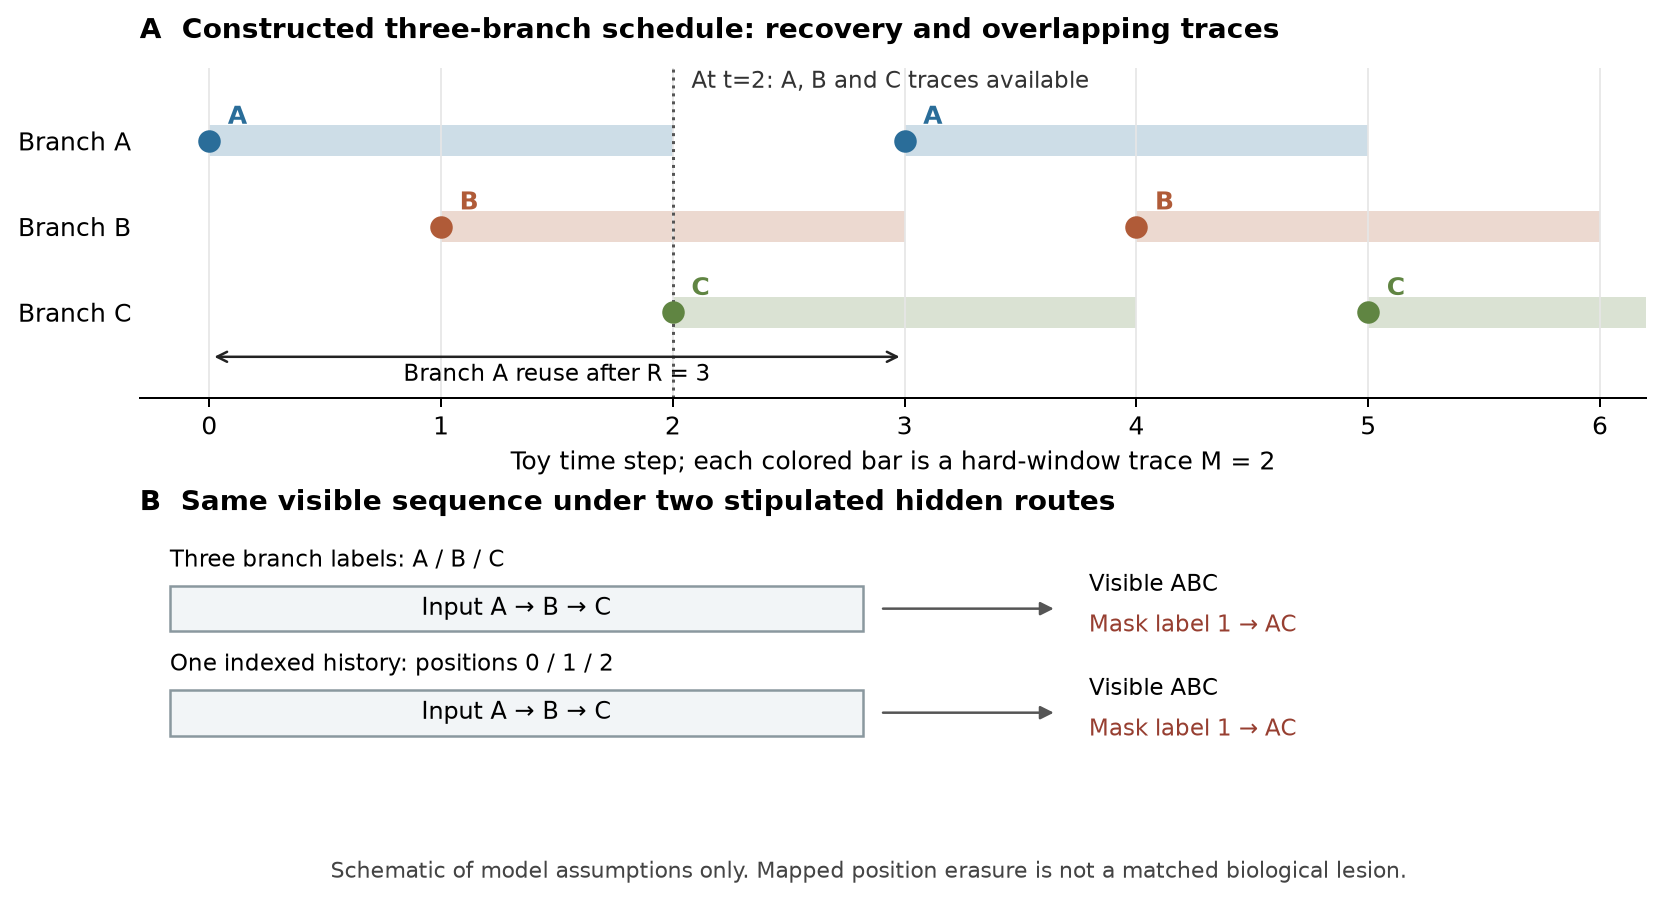
\includegraphics[keepaspectratio,alt={Constructed schedule and route-equivalence schematic. Panel A depicts hard-window traces for three abstract branches, R=3 and M=2; panel B shows two hidden routes with the same visible ABC and the same AC after stipulated logical label-1 erasure. This is explanatory model output, not measured dendritic activity or a matched biological lesion.}]{figures/schedule-and-identification.png}}
\caption{Constructed schedule and route-equivalence schematic. Panel A depicts hard-window traces for three abstract branches, R=3 and M=2; panel B shows two hidden routes with the same visible ABC and the same AC after stipulated logical label-1 erasure. This is explanatory model output, not measured dendritic activity or a matched biological lesion.}
\end{figure}

The \href{https://github.com/v5ma/v5ma.github.io/blob/f6d3867df89ae9dea32f763b1d55c84212c41cc6/papers/companions/five-papers-20260923/temporal/paper/figures/FIGURE-PROTOCOL-20260923.md}{figure protocol} declares every value and marks the mapped erasure as a logical control only. It visualizes both the conditional schedule and the identification limit; it cannot adjudicate cellular experience.

\subsubsection{5.4 Local content states expose an exact aggregation boundary}\label{local-content-states-expose-an-exact-aggregation-boundary}

The \href{https://github.com/v5ma/v5ma.github.io/blob/f6d3867df89ae9dea32f763b1d55c84212c41cc6/papers/companions/five-papers-20260923/temporal/paper/applications/local-content-v05/PROTOCOL.md}{fifth application and frozen protocol} replaces the symbol-history readout with explicit compartment states. For two, three or four abstract receiving components, constant drive, pairwise inhibition and local adaptation determine continuous rate activation. An Euler step of 0.002 approximates fast activation with time constant 0.05 and adaptation with time constant 0.8. Drive is 1, mutual inhibition is 2, and adaptation strength is 1.7. These are dimensionless construction parameters, not estimates of dendritic physiology. Small fixed asymmetric initial conditions break permutation symmetry. No branch-index scheduler or winner-take-one operation selects a contributor.

After twelve settling units, the fixed six-unit observation window contains 6, 8 and 9 changes of the most active component for the two-, three- and four-component baseline. Removing adaptation or pairwise coupling eliminates those switches in this window. A recovery-heterogeneity condition gives 6, 8 and 8 changes. Such rate-dominance changes are not measured spikes or proof of a stable limit cycle, and the number three has no privileged status in this construction.

At an input event, normalized nonnegative activation allocates a total content write of one across the compartments. Each contains two four-coordinate content matrices with decay times 0.4 and 1.6. The input explicitly gives an object label and feature label; their outer product supplies the conjunction to be retained. Thus the model preserves provided ownership, rather than solving segmentation or discovering binding from an ambiguous scene. Between events these local states decay, so retained earlier content---not a global timestamped list---contributes to the next readout. A fixed downstream rule uses the summed fast and slow traces to select an order-dependent action port; another compares diagonal and crossed object-feature conjunctions.

The \href{https://github.com/v5ma/v5ma.github.io/blob/f6d3867df89ae9dea32f763b1d55c84212c41cc6/papers/companions/five-papers-20260923/temporal/paper/applications/local-content-v05/README.md}{complete result and readback} cross component count, four dynamical variants, five gaps, three delays, two input orders and two ownership assignments. All 576 separated-event cases produce the declared order-dependent action, and all 144 simultaneous cases mark order as unavailable. All 720 cases preserve supplied ownership. These are exhaustive cases of this small grid, not 720 independent experiments. The two-event order rule is not claimed for arbitrary delays, noisy sequences, learned behavior or full episodes. The independent-marginals control cannot distinguish the two ownership assignments because their separate object and feature counts are identical; it is deliberately weaker than a recurrent memory.

The decisive control is stronger and adverse to a necessity claim. For each of the two time constants, write the local trace as \(h_i\), normalized allocation as \(w_i\), and the aggregate as \(H=\sum_i h_i\). Between events and at event time \(t\),

\[
\dot h_i=-h_i/\tau,\qquad h_i(t^+)=h_i(t^-)+w_i(t)x_t,\qquad \sum_i w_i(t)=1. \tag{7}
\]

\textbf{Proposition 4 (linear local-trace aggregation).} With equal trace decay across compartments and zero initial traces, the summed-local model and a single ordinary state bank satisfying

\[
\dot H=-H/\tau,\qquad H(t^+)=H(t^-)+x_t \tag{8}
\]

have identical aggregate states for every finite event sequence. Consequently any declared downstream rule using only those aggregates has identical outputs.

\textbf{Proof.} Summing the between-event equations yields \(\dot H=-H/\tau\). Summing the increments yields \(x_t\) because the weights sum to one. The initial sums agree. Uniqueness of exponential decay between each pair of events and induction through the shared increments prove equality. The same reasoning applies separately to both time constants. Nonnegative normalized activation is one allocation rule; the result does not depend on how that allocation is generated. \(\blacksquare\)

The ordinary nonoscillatory bank agrees with the saved local sums to at most \(2.22\times10^{-16}\). Removing adaptation or coupling changes the allocation dynamics but not the declared task outputs. Erasing retained content removes the order decision; restoring the saved state restores it. The \href{https://github.com/v5ma/v5ma.github.io/blob/f6d3867df89ae9dea32f763b1d55c84212c41cc6/papers/companions/five-papers-20260923/temporal/paper/applications/local-content-v05/AUDIT.json}{separate audit} directly reconstructs event kernels, checks partial-compartment erasure, and confirms byte-identical replay. Its 3,602 arithmetic checks are implementation evidence, not scientific effect sizes. The model contains no behavioral environment in which these ports generate a further sensed consequence, and no source-fitted oscillatory reference for a physiological PWD claim.

\begin{figure}
\centering
\pandocbounded{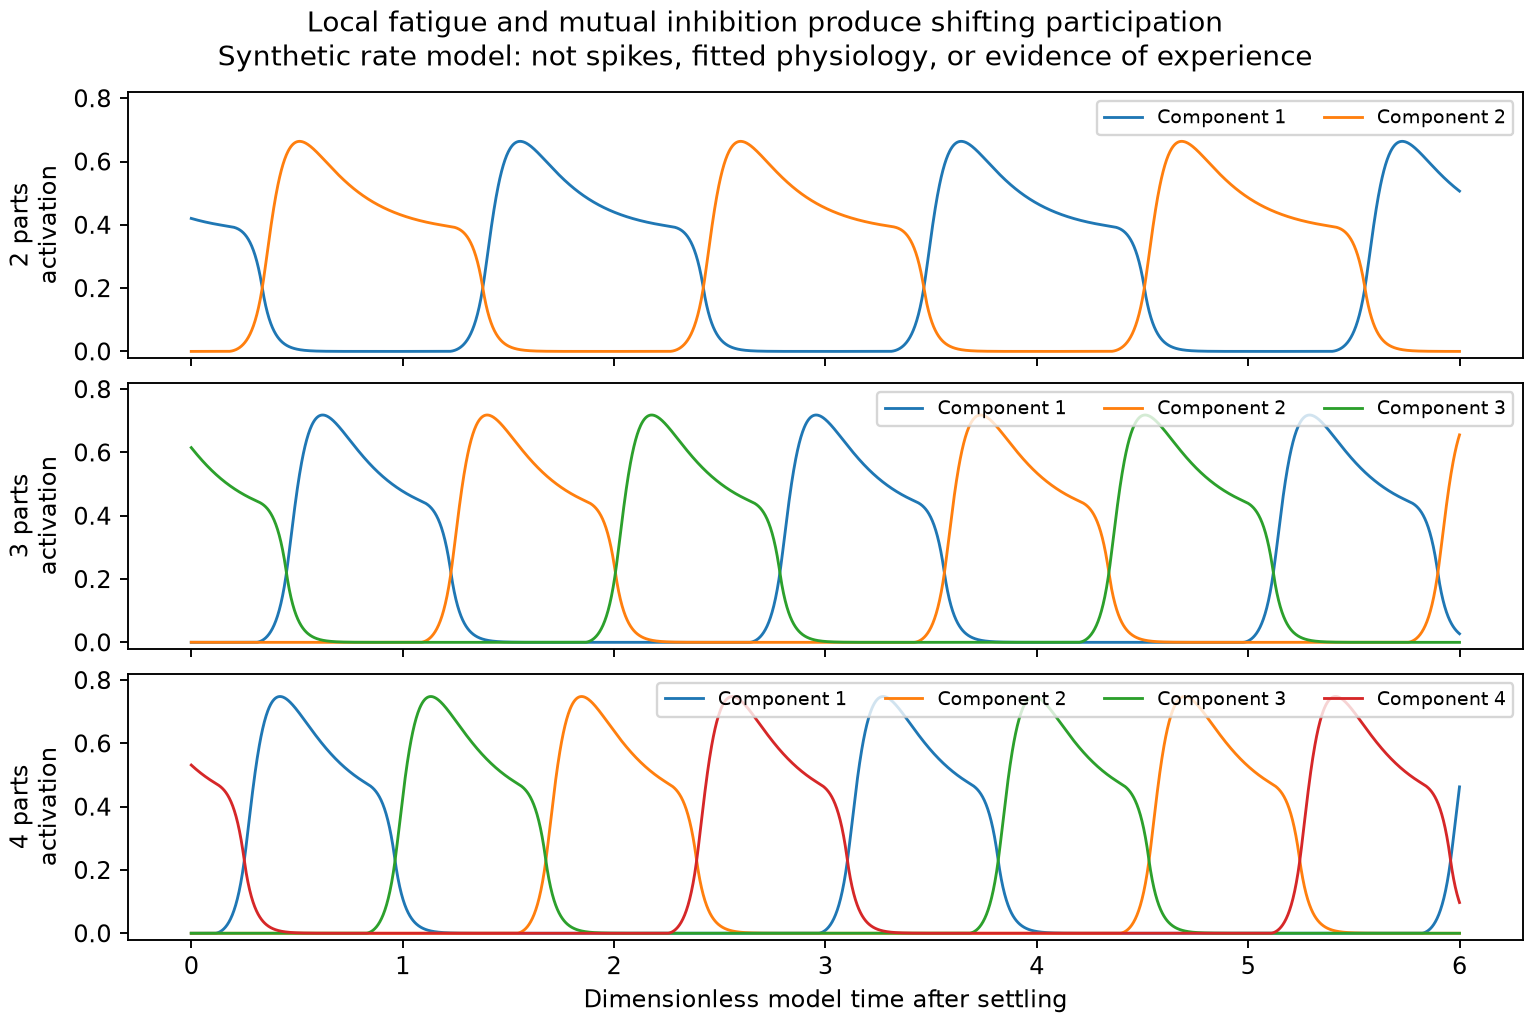
\includegraphics[keepaspectratio,alt={Synthetic local activation under constant drive, adaptation and mutual inhibition. Two, three and four components show changing participation without an assigned branch schedule. Content is represented separately in local decaying matrices. Removing adaptation or coupling changes these dynamics but not this application's aggregate downstream decisions. These are model rates, not dendritic spike recordings.}]{figures/local-content-dynamics.png}}
\caption{Synthetic local activation under constant drive, adaptation and mutual inhibition. Two, three and four components show changing participation without an assigned branch schedule. Content is represented separately in local decaying matrices. Removing adaptation or coupling changes these dynamics but not this application's aggregate downstream decisions. These are model rates, not dendritic spike recordings.}
\end{figure}

This result improves the construction while limiting its interpretation. Local content and a usable action readout are implemented, but alternation is not functionally necessary for these aggregate endpoints. A stronger candidate needs an independently justified operation that prevents the aggregation---such as branch-specific downstream reception, saturating local storage or measured heterogeneous content decay---and a comparably informed state-based alternative. Adding a special rule merely to force an advantage would not establish the biological explanation. The result does not reject the physical possibility of alternating dendritic participation; it identifies exactly why this experiment does not demonstrate its distinctive causal contribution.

\subsubsection{5.5 Three conditional constraints on temporal selection}\label{three-conditional-constraints-on-temporal-selection}

The following elementary results clarify the comparison; they are not fits to the Hesse recordings and do not add a sixth learned or physiological application. The accompanying fixed arithmetic fixtures check particular consequences without recreating the preprint's analysis.

\textbf{Proposition 5 (state pooling can erase a contrast without erasing state structure).} Let a population vector have conditional means μC = b + gC a and μS = b - gS a, with occupancy p for C and 1-p for S, nonnegative gains gC,gS and finite conditional covariance matrices ΣC,ΣS. Its pooled mean and covariance are

\[
\bar\mu=b+[p g_C-(1-p)g_S]a,\qquad
\operatorname{Cov}(R)=p\Sigma_C+(1-p)\Sigma_S+p(1-p)(\mu_C-\mu_S)(\mu_C-\mu_S)^T. \tag{9}
\]

If p gC = (1-p)gS, the mean contrast vanishes, but the between-state covariance term remains whenever 0 \textless{} p \textless{} 1 and μC differs from μS.

\textbf{Proof.} The mean follows by conditioning on the state. The law of total covariance splits the conditional covariance average from the covariance of the two conditional means; substituting their deviations from the pooled mean gives the last term. The stated cancellation removes only the first moment along a. It does not equate the full distribution to a constant-rate model. \(\blacksquare\)

This is a population-vector identity, not a derivation of the preprint's nonlinear modulation index or its reported regression slopes. It explains why averaging can conceal a strong conditional contrast while held-out covariance, state-conditioned responses and temporal likelihood remain informative. If the entries of a sum to zero and the baseline is sufficiently positive, the total mean firing can also stay fixed while the represented contrast changes. Thus a total-rate match does not imply an information match.

\textbf{Proposition 6 (alternation need not supply an oscillatory phase).} Consider a stationary symmetric continuous-time two-state Markov process S(t) in \{-1,+1\}, switching with constant hazard λ \textgreater{} 0. Its mean dwell is 1/λ and

\[
\mathbb E[S(t)S(t+\tau)]=e^{-2\lambda|\tau|},\qquad
P(\omega)=\frac{4\lambda}{4\lambda^2+\omega^2}. \tag{10}
\]

Here P is the two-sided Fourier transform of the unit-variance autocorrelation under the angular-frequency convention. It has its maximum at zero frequency, not a nonzero oscillatory peak.

\textbf{Proof.} If m(τ) is the expected state conditional on S(0)=1, the transition generator gives m'(τ) = -2λm(τ), with m(0)=1. Symmetry and stationarity give the displayed correlation. Integrating its even exponential Fourier transform gives P. For positive ω, the denominator strictly increases, so P strictly decreases. \(\blacksquare\)

This is a standard two-state-process identity; its exponential correlation is also used explicitly in Hesse et al.'s autocorrelation Methods {[}20{]}, not introduced here as new mathematics. The counterexample does not show that the brain lacks an oscillator, or that a fitted HMM proves a Markov mechanism. It shows why a pattern of alternation alone cannot identify one. In this model the correlation-decay constant is half the mean dwell and the median dwell is log(2)/λ; these are distinct quantities. The preprint's Methods identify D=67 ms as a mean dwell, corresponding to an exponential-model median of about 46 ms, while its main text calls 67 ms a time constant. I therefore do not equate that parameter with its separate 64/59-ms HMM medians or use any of them as a fitted SAN parameter. A future reanalysis should preserve the exact parameter convention.

\textbf{Proposition 7 (a conditional gap bound for retained usability).} Suppose a receiver's selected content trace has amplitude H0 immediately after an effective refresh, decays as H(t)=H0 exp(-t/τh) between refreshes, and supports a declared functional readout exactly while H ≥ θ, where H0 ≥ θ \textgreater{} 0 and τh \textgreater{} 0. Across a gap G ≥ 0, that readout remains available if and only if

\[
G\leq\tau_h\log(H_0/\theta). \tag{11}
\]

\textbf{Proof.} Substitute the decay solution into H(G) ≥ θ, divide by positive H0, take logarithms and rearrange. For a random gap, the probability of preserving this specified readout is the gap-distribution probability below the same bound. \(\blacksquare\)

This predicts an observable timing boundary only after the trace, its refresh rule and the readout threshold have been independently justified. H0 is the measured post-refresh level, not an unexplained automatic reset. No claim is made that crossing θ defines phenomenal consciousness. The result gives the continuity proposal a testable form: locally interrupted representation could support continuing downstream use when the selected trace lasts through its gaps, while sufficiently long gaps should impair that specific use. Neither the relevant trace nor such a boundary was measured in the Hesse preprint. A nonoscillatory memory can satisfy the same bound and remains a necessary comparator.

This connects to the aggregation boundary in Section 5.4. A fixed linear readout of the same summed traces, or a common gain applied to that sum, retains the state-bank equivalence. A content- or compartment-specific receiving rule requires information that the bare aggregate discarded. Its presence, physical targeting and acquisition must be measured rather than supplied only to the favored model. A nonoscillatory comparator given the same state/content information may implement the same selection. Temporal selection is therefore a mechanistic candidate to identify, not an advantage established by adding an assumed gate.

\subsection{6. Discriminating experiments}\label{discriminating-experiments}

The first biological test would choose a specified cell type and preparation, identify branches and input sites, and measure branch activity, recovery and any retained trace independently before predicting a new stimulation condition. Reverse input order while matching input number and amplitude. Compare simultaneous, staggered and irregular schedules. A result must report local events, soma and axonal output separately; back-propagation can change the whole tree after one branch contributes. Park et al.'s measured alternation and broadly expressed distal spikes {[}11{]} make a direct comparison mandatory: does a candidate branch sequence preserve ordered \emph{content} beyond their channel-availability account, or merely rename alternating spike propagation? Wu et al.'s in-vivo CA2 result {[}16{]} makes local-versus-somatic event assignment an additional mandatory control. Their and Park et al.'s reported event windows must not be silently inserted as this model's distinct recovery \texttt{R} and content-lifetime \texttt{M} parameters.

The causal test would perturb the proposed alternation or recovery route and ask whether sequence/interval discrimination changes beyond the effect expected from a general reduction in activity. The mapped-erasure control in §5.3 shows why route labels alone are insufficient: the perturbation must be independently localized in tissue, with lost content and broad excitability measured rather than assumed away. Rescue would restore the relevant relationship while controlling total input and output as closely as the preparation permits. A claimed \emph{k}-way overlap should predict an interval range from independently estimated trace and recovery parameters, not be fitted after every outcome is known.

The network test would ask whether a later receiver actually uses the preserved relation. For example, distinct ordered inputs could predict different next observations or actions under the same component counts. Selectively disconnect the proposed route while retaining decodable upstream information; if behavior is unchanged, upstream decodability did not establish the claimed functional join. Controls must include a nonoscillatory state-dependent network, a flexible recurrent model, a matched-rate model, and a direct sensory-cue check.

For a fly application, use cell- and species-specific timing and anatomy. The known phase-splayed flight motor circuit is a comparison, not proof that fly sensory dendrites instantiate this model. A calcium-imaging sample rate must not be described as a neural clock or phase measurement without adequate temporal resolution.

\subsubsection{6.1 A state-resolved network extension}\label{a-state-resolved-network-extension}

The new preprint motivates a second, complementary assay without replacing the branch experiment. Begin with independent stimulus templates and held-out neurons, trials and sessions. First establish that the relevant content distinction is reproducible; then compare flexible continuous-state and correlated-noise alternatives as well as discrete switches. Report nesting by animal, session and stimulus pair rather than treating thousands of cell-stimulus combinations as thousands of independent subjects. The current two-animal evidence is not a species-wide prevalence estimate.

For a receiver-use test, record source content and a prespecified downstream endpoint together. State assignment must not use that endpoint, its later behavioral answer, or the spikes whose selectivity it will test. A decoder intended to trigger a perturbation must use only past and present observations, with latency and error calibrated independently. The preprint's Viterbi sequence inference is retrospective, and its 66\% state-discrimination assay classifies the order of paired state-resolved responses; neither alone establishes an implementable online state detector. Offline reconstruction is still useful, but it answers a different question.

Three outcomes would discriminate concrete mechanisms. First, a localized perturbation that changes a receiving window while preserving decodable source content should selectively alter the nominated downstream contribution. Preserve comparable delivered stimulation and audit firing, tuning, arousal and sampling side effects; an unmatched loss of input is not a timing-specific result. Second, independently estimated retained-content decay should predict failures across imposed or naturally variable gaps in selected input, including conditions not used for fitting. Third, if a phase-specific account is proposed, the measured source-reference-receiver relationship should predict the result beyond content-state labels and a nonoscillatory state-dependent comparator. A state effect without this added evidence supports temporal selection but not the specific PWD realization.

For the separately declared state-conditional perturbation assay, randomize interventions within pre-intervention state/history strata, retain all assignments and report state-estimation uncertainty and failed deliveries. This conditional effect is distinct from the total effect of a scheduling policy assigned before eligibility; report that policy effect separately when such a policy is tested. Post-intervention state occupancy is an outcome or candidate mediator, not a harmless selection filter. Test regional lags using preregistered alignment rules rather than assuming that every patch occupies the same state simultaneously. A null after failed targeting is inconclusive; a precise null after verified targeting challenges the declared route. Successful downstream use still does not by itself establish elementary cellular experience.

\subsection{7. Temporal experience is an additional hypothesis}\label{temporal-experience-is-an-additional-hypothesis}

I propose two possible interpretations that the functional mechanism alone cannot decide. On a network-level account, branch and population timing contribute to the experience of the organized whole; an individual branch or neuron need not itself be an experiencing subject. On a stronger cellular account, a cell's organized succession might already have a minimal temporal experience. My pixel analogy is meant to keep that question visible, not to prove it. A changing pixel can contribute to a display without being a viewer of the display.

The stronger account owes two explanations: what distinguishes an experiencing cell from any other history-dependent physical device, and how any elementary experiences relate to an organism's one experienced world. Combining signals is not yet combining subjects. Functional tests can constrain the candidate physical organization while leaving the phenomenal interpretation underdetermined. The paper should not relabel a successful order classifier as evidence that a neuron feels time pass.

\subsection{8. Scope, falsification and limits of the draft}\label{scope-falsification-and-limits-of-the-draft}

A specified mechanistic prediction can be rejected if independently estimated recovery and trace parameters predict a timing or interference range that a sufficiently sensitive controlled test excludes, or if a localized perturbation fails to produce the predeclared downstream effect despite verified target engagement and adequate precision. Measurement failure, absent target engagement or an underpowered null is inconclusive, not automatic falsification. A failure of that specified implementation would not by itself decide the broader SAN theory or the philosophical experience claim.

An equally fitting nonoscillatory model has a different implication: it shows that the available observations do not identify the physical implementation, or that no unique performance advantage has been demonstrated. It does \textbf{not} establish that the proposed branch organization is absent. This distinction follows directly from the passive-I/O and mapped-erasure results in Sections 5.2--5.3. A symbolic history buffer can reproduce an observable without measuring the biological route. Conversely, a successful temporal-ensemble toy does not establish that the brain uses it. The next test must distinguish a rejected prediction, unresolved implementation identity, and absent performance advantage rather than combine them into one verdict.

This preprint retains four earlier source-specific ancestors and one derivative witness, with the 2011 note's 2023 appendix separated, and adds the three 2022 records in Section 1.1. Its version-pinned adjacent-paper comparison narrows the ownership claim to the proposed compartmental join; it is targeted rather than an exhaustive SAN-corpus audit. The historical claim therefore reaches only the original passages actually inspected. The current finite applications deliberately lack independently measured branch parameters, physiological noise, physical route-targeting and a matched learned recurrent implementation. They establish conditional feasibility and nonidentification, not a positive dendritic mechanism. Those are prospective experiments and comparator requirements, not hidden accomplishments of this draft. The triplet remains an author-proposed candidate, not an anatomical law. The passive and mapped-intervention proofs do not replace tissue measurements or a physically matched perturbation. No conclusion about elementary experience follows from any present test. Author-authorized preprint publication does not resolve that additional hypothesis or substitute for independent scientific review.

\begingroup\small
\subsection{References}\label{references}

\begin{enumerate}
\def\labelenumi{\arabic{enumi}.}
\item
  Branco T, Clark BA, Häusser M. Dendritic discrimination of temporal input sequences in cortical neurons. \emph{Science}. 2010;329:1671--1675. \href{https://doi.org/10.1126/science.1189664}{DOI}.
\item
  Remy S, Csicsvari J, Beck H. Activity-dependent control of neuronal output by local and global dendritic spike attenuation. \emph{Neuron}. 2009;61:906--916. \href{https://pubmed.ncbi.nlm.nih.gov/19323999/}{PubMed}.
\item
  Larkum ME, Zhu JJ, Sakmann B. A new cellular mechanism for coupling inputs arriving at different cortical layers. \emph{Nature}. 1999;398:338--341. \href{https://doi.org/10.1038/18686}{DOI}.
\item
  Hürkey S, et al.~Gap junctions desynchronize a neural circuit to stabilize insect flight. \emph{Nature}. 2023;618:118--125. \href{https://doi.org/10.1038/s41586-023-06099-0}{DOI}.
\item
  Karmarkar UR, Buonomano DV. Timing in the absence of clocks: encoding time in neural network states. \emph{Neuron}. 2007;53:427--438. \href{https://pubmed.ncbi.nlm.nih.gov/17270738/}{PubMed}.
\item
  Blumberg M. Note/comment thread dated 19 April 2012, \texttt{a0632z.md}, preserved in the author's SAN source archive. Current copy and hash in the accompanying source ledger. Unpublished source, not an independently verified public-priority date.
\item
  Blumberg M. Note dated 18 September 2012, \texttt{a0119z.md}, preserved in the author's SAN source archive. Current copy and hash in the accompanying source ledger. Unpublished source, not an independently verified public-priority date.
\item
  Blumberg M. Undated SAN note, \texttt{a0049z.md}, preserved by 2022 in the author's source archive. Current copy and hash in the accompanying source ledger. Its speculative analogies are not imported as scientific support.
\item
  Blumberg M. Note internally dated 21 September 2011, \texttt{a0051z.md}, preserved in the author's SAN source archive. The separately appended January 2023 excerpt is excluded from the 2011 claim. Current copy and hash in the accompanying source ledger; owner-stated composition date is distinct from later Git fixation.
\item
  Blumberg M. \texttt{a0072z.md}, a later cutlet compilation describing dialogue before 21 September 2011. Its overlapping passages are not treated as an independent contemporaneous witness. Current copy and hash in the accompanying source ledger.
\item
  Park P, et al.~Dendritic excitations govern back-propagation via a spike-rate accelerometer. \emph{Nature Communications}. 2025;16:1333. \href{https://doi.org/10.1038/s41467-025-55819-9}{Primary article}.
\item
  Blumberg M. \emph{The Tonic Canvas of Consciousness}. Public Paper 75, author-held PDF version checked in the accompanying ownership readback. Cited here for prior SAN scope, not independent empirical confirmation.
\item
  Blumberg M. \emph{The Learning Loop That Learns Itself}. Draft 10, 13 August 2026. Cited here for prior SAN scope and source genealogy; its own bounded application limits are preserved.
\item
  Blumberg M. \emph{Neural Rendering Composition and Granularity Tuning}. Working Draft 6, 22 September 2026. Cited here for adjacent manuscript ownership, not as independent physiological evidence.
\item
  Blumberg M. \emph{Self-Aware Networks in a Connectome-Constrained Fly Brain}. Working Draft 22, 22 September 2026. Cited here for adjacent species-specific scope, not as proof of dendritic or experiential claims.
\item
  Wu X, Lee BH, Park P, et al.~\emph{A dendrite-resolved, in vivo transfer function from spike patterns to dendritic Ca2+}. bioRxiv preprint, 2026. \href{https://www.janelia.org/publication/a-dendrite-resolved-in-vivo-transfer-function-from-spike-patterns-to-dendritic-ca2}{Authors' publication abstract}; \href{https://doi.org/10.64898/2026.01.18.700189}{preprint DOI}. Abstract-level comparator only; not peer-reviewed at this checked version.
\item
  Lisman JE, Idiart MAP. Storage of 7 ± 2 short-term memories in oscillatory subcycles. \emph{Science}. 1995;267:1512--1515. \href{https://doi.org/10.1126/science.7878473}{DOI}.
\item
  Rabinovich M, Volkovskii A, Lecanda P, Huerta R, Abarbanel HDI, Laurent G. Dynamical encoding by networks of competing neuron groups: winnerless competition. \emph{Physical Review Letters}. 2001;87:068102. \href{https://doi.org/10.1103/PhysRevLett.87.068102}{DOI}.
\item
  Cichon J, Gan WB. Branch-specific dendritic Ca2+ spikes cause persistent synaptic plasticity. \emph{Nature}. 2015;520:180--185. \href{https://doi.org/10.1038/nature14251}{DOI}.
\item
  Hesse JK, Lanfranchi FF, McGrory C, Shi Y, Engel TA, Tsao DY. Rapid alternation of conscious and suppressed stimulus representations in the primate brain. bioRxiv, v1 posted 16 October 2026. Not peer reviewed. \href{https://doi.org/10.64898/2026.10.15.759299}{Primary preprint}.
\item
  Hesse JK, Tsao DY. A new no-report paradigm reveals that face cells encode both consciously perceived and suppressed stimuli. eLife. 2020;9:e58360. \href{https://doi.org/10.7554/eLife.58360}{DOI}.
\item
  She L, Benna MK, Shi Y, Fusi S, Tsao DY. Temporal multiplexing of perception and memory codes in IT cortex. Nature. 2024;629:861-868. \href{https://doi.org/10.1038/s41586-024-07349-5}{DOI}.
\item
  Blumberg M. Learning to Feel: Perception-Action Learning, Phase-Compatible Recruitment, and Conscious Sensory Access in Self-Aware Networks. Public preprint v1.2, 20 October 2026. \href{https://doi.org/10.5281/zenodo.23509961}{This version}; \href{https://doi.org/10.5281/zenodo.23455801}{preserved v1.1}; \href{https://doi.org/10.5281/zenodo.23447925}{preserved v1.0}.
\item
  Blumberg M. Oscillation is just for the canvas of consciousness. Rough recording transcript, \texttt{b0192y\ ctpr.txt}, 04:04. Commit-dated 8 June 2022; underlying recording catalogued 17 September 2021. \href{https://github.com/v5ma/selfawarenetworks/blob/09b8306fbb54536e20ba1071e91dff0cb8a4770f/b0192y\%20ctpr.txt\#L21}{Exact transcript}.
\item
  Blumberg M. Detection/rendering synthesis in \texttt{0abstractbump.md}, line 13. Commit-dated 28 November 2022. \href{https://github.com/v5ma/selfawarenetworks/blob/4e0cf1ee0975c01dc57182368497d3f0cd864030/0abstractbump.md\#L13}{Exact source}.
\item
  Blumberg M. NAPOT 6, \texttt{a0325zNAPOT6.md}, lines 99-133. Commit-dated 28 November 2022. \href{https://github.com/v5ma/selfawarenetworks/blob/4e0cf1ee0975c01dc57182368497d3f0cd864030/a0325zNAPOT6.md\#L99}{Exact historical version}. Historical theory, not an independent physiological result.
\end{enumerate}

\endgroup
\begingroup\small\par\smallskip\noindent\textbf{Version provenance.}\label{successor-provenance} Version 1.2 adds a focused historical-source update with AI assistance. Its companion includes exact source locators and date distinctions alongside the unchanged v1.1 arithmetic checks; the v1.0 companion retains the original applications. Existing numerical results and both earlier public versions are unchanged. Publication is not independent peer review.

\endgroup
\end{document}
